\section{CPU Parallelization}
The given CPU sequential code can be optimized with an
OpenOMP\footnote{http://openmp.org/} pragma. In the outmost \textbf{outer} loop
in \textbf{run\_OrigCPU} we can privatize the \emph{strike} and \emph{globs}
variables, and add the OpenOMP pragma to CPU parallelize the loop. The code
transformation is safe as \emph{strike} and \emph{globs} are not used accross
iterations. Furthermore the outer loop is itself parallelisable as there are
no cross iteration dependencies. Each loop iteration independently computes a
single value of the final result.

Figure \ref{fig:openOMP} shows how the pragma is used.
\begin{figure}[!ht]
\centering
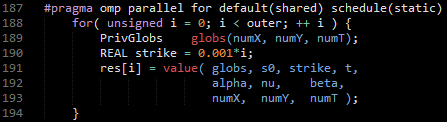
\includegraphics[scale=1]{input/figures/openOMPCPU.png}
\caption{Use of openOMP pragma to achieve CPU parallelization.\label{fig:openOMP}}
\end{figure}

When timing the OpenOMP version the code averages on $257131\mu s \approx 2.5s$
when run with the small data set, $331305\mu s \approx 3.3s$ with the medium
data set and $13600746\mu s \approx 13.6s$ with the large data set.
Hence these shall be our benchmark requirements for our CUDA version.
